\documentclass{beamer}


\usepackage{graphicx}
\usepackage{amsmath}
\usepackage{mathdots}
\usepackage{amsthm}
\usepackage{amssymb}
\usepackage{pstricks}
\usepackage{pst-node}
\pagenumbering{arabic}
\usepackage{hyperref}
\usepackage{lscape}
\usenavigationsymbolstemplate{}
\definecolor{slidetitlecolor}{RGB}{51,0,102}
\setbeamercolor{frametitle}{fg=slidetitlecolor}
\definecolor{item1color}{RGB}{51,153,255}
\setbeamercolor{itemize item}{fg=item1color}
\setbeamertemplate{itemize item}[circle]
\setbeamercolor{enumerate item}{fg=item1color}





\begin{document}


\frame{
\begin{center}
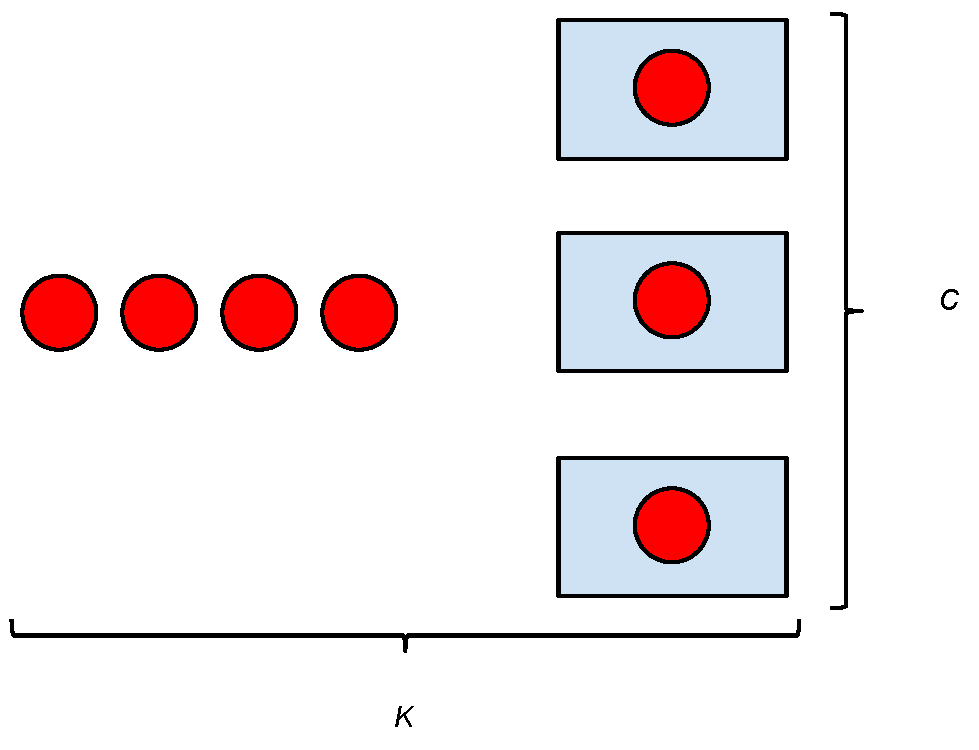
\includegraphics[width=10cm]{MMcK_Queue_Diagram.pdf}
\end{center}
}

\frame{\frametitle{Classification of queues}
There is a classification scheme for commonly encountered queues (originally devised by David Kendall). A general queue is denoted:
$$A/B/c/K$$
where we make the following assumptions:
\begin{enumerate}
\item Inter-arrival times are independent and give by some distribution $A$.
\item Service times are independent and given by some distribution $B$.
\item There are $c$ servers.
\item There is a buffer of size $K$.\end{enumerate}
}

\frame{\frametitle{$M/M/c/K$}
\begin{center}
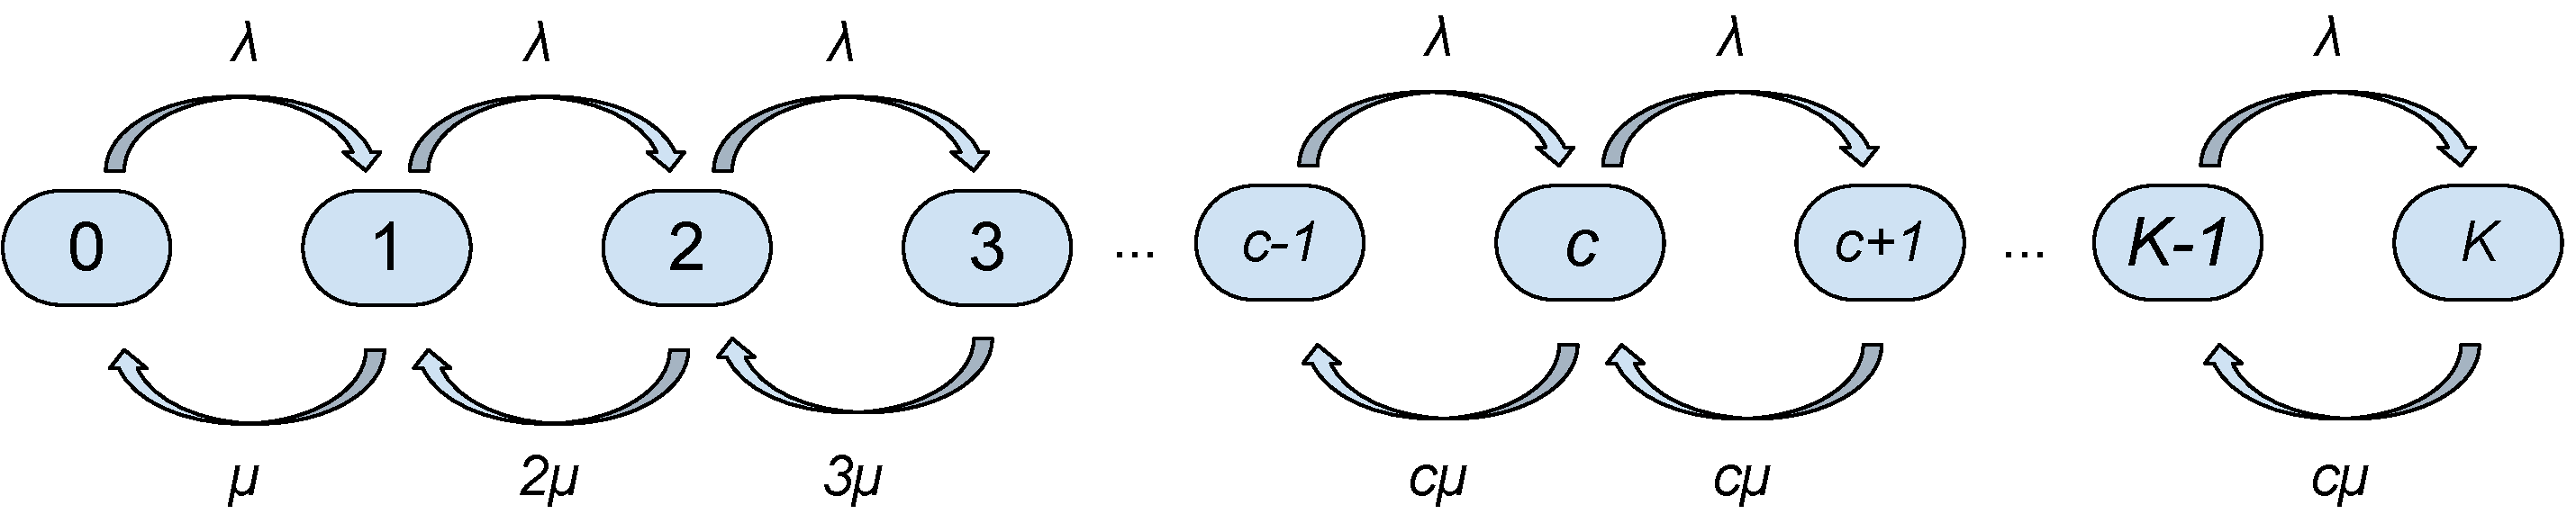
\includegraphics[width=11cm]{MMcK.pdf}
\end{center}
}


\frame{\frametitle{$M/M/c/K$}
Probability that we have $0\leq i\leq K$ customers in system: $\pi_i$.
$$\pi_i=\left\{\;\begin{array}{@{}c@{}}
{\left(\lambda\over\mu \right)^i\over i!}\pi_0\text{ for }i\leq c\\[2mm]
{\left(\lambda\over\mu \right)^i\over c!c^{i-c}}\pi_0\text{ for }i> c\\[2mm]
\end{array}
\right.$$
We then set $\sum_{i=0}^{K}\pi_i=1$ to get $\pi_0$.
}

\end{document}
